\documentclass{article}
\usepackage[magyar]{babel}
\usepackage[utf8]{inputenc}
\usepackage[T1]{fontenc}
\usepackage{amsfonts}
\usepackage{amssymb}
\usepackage{amsthm}
\usepackage{color}
\usepackage{mathtools}
\usepackage{algorithm}
\usepackage{algorithmicx}
\usepackage{algpseudocode}
\usepackage{listings}
\usepackage{multirow}
\usepackage{pgfplots}
\usepackage{tikz-qtree}

\lstset{literate=
  {á}{{\'a}}1 {é}{{\'e}}1 {í}{{\'i}}1 {ó}{{\'o}}1 {ú}{{\'u}}1
  {Á}{{\'A}}1 {É}{{\'E}}1 {Í}{{\'I}}1 {Ó}{{\'O}}1 {Ú}{{\'U}}1
  {à}{{\`a}}1 {è}{{\`e}}1 {ì}{{\`i}}1 {ò}{{\`o}}1 {ù}{{\`u}}1
  {À}{{\`A}}1 {È}{{\'E}}1 {Ì}{{\`I}}1 {Ò}{{\`O}}1 {Ù}{{\`U}}1
  {ä}{{\"a}}1 {ë}{{\"e}}1 {ï}{{\"i}}1 {ö}{{\"o}}1 {ü}{{\"u}}1
  {Ä}{{\"A}}1 {Ë}{{\"E}}1 {Ï}{{\"I}}1 {Ö}{{\"O}}1 {Ü}{{\"U}}1
  {â}{{\^a}}1 {ê}{{\^e}}1 {î}{{\^i}}1 {ô}{{\^o}}1 {û}{{\^u}}1
  {Â}{{\^A}}1 {Ê}{{\^E}}1 {Î}{{\^I}}1 {Ô}{{\^O}}1 {Û}{{\^U}}1
  {œ}{{\oe}}1 {Œ}{{\OE}}1 {æ}{{\ae}}1 {Æ}{{\AE}}1 {ß}{{\ss}}1
  {ű}{{\H{u}}}1 {Ű}{{\H{U}}}1 {ő}{{\H{o}}}1 {Ő}{{\H{O}}}1
  {ç}{{\c c}}1 {Ç}{{\c C}}1 {ø}{{\o}}1 {å}{{\r a}}1 {Å}{{\r A}}1
  {€}{{\euro}}1 {£}{{\pounds}}1 {«}{{\guillemotleft}}1
  {»}{{\guillemotright}}1 {ñ}{{\~n}}1 {Ñ}{{\~N}}1 {¿}{{?`}}1
}

\pgfplotsset{compat=1.9}

\begin{document}

\tableofcontents

\section{Bevezető}

Ez a doksi azért van, hogy magamnak is, és neked is összefoglaljam, hogy az edénysoros szita sebessége hogyan jött ki.
Az eredeti kérdés, amivel megtaláltalak, valami olyasmi volt, hogy hogyan lehet jól szitálni funkcionálisan.

Nagyon meglepő dolgokat nem kell majd számolni.
Az egész bizonygatás arra fog kimenni, hogy elsüthessük Mertens tételét.
Ehhez végig kell gondolni, hogy:
\begin{itemize}
\item Implementálni lehet úgy ezt a szitát, hogy láncolt listákat és rekurziót használ, és a műveletek száma arányos az összeadások közben megváltozott számjegyek számával.

\item Ha egy $p$ számot $k$-szor összeadunk önmagával a számjegyenkénti összeadással, akkor a számítás alatt megváltozott számjegyek száma arányos $k\log{p}$-vel.

\item A műveleteket nem a végrehajtás sorrendjében számoljuk össze, hanem minden művelet hozzáköthető ahhoz hogy
\begin{itemize}
\item a sor pozícióját növeljük $n$-szer $1$-gyel

\item vagy egy $p$ prím pozícióját növeljük $p$-vel $\frac{n}{p}$-szer.
\end{itemize}

\item Az előző szétcincálásból csinálunk egy végső összeget.

\item Használjuk Mertens tételét.

\item Az eredmény remélhetőleg az, hogy az $n$-ig szitálás futási ideje $\Theta(n \log{n})$.
\end{itemize}

Ennek a doksinak a formája chitchat, és a "vegyük észre, hogy ..." lesz a legfontosabb módszer.
A gyanúsabb helyeken szükség szerint bővíthetem.

\section{Edénysor elejének eltávolítása}

A szakdolgozat jelöléseit használva legyen
\begin{align*}
r &\in b(q, d(p(q), p(r))) \\
d' &= d(p(q), p(r)) \\
k &= h(p(q), p(r))
\end{align*}
Ekkor $d$ definíciója miatt
\begin{align*}
k = \left\lfloor \frac{d'}{a-1} \right\rfloor \\
\forall i > k: p(r)_i &= p(q)_i \\
p(r)_k &= d'+1-(a-1)k
\end{align*}
Azaz a $d'$ edényben lévő elemek számjegyeit az alsó $k$ helyiértéket leszámítva ismerjük.
Ezeket tárolni sem szükséges.

Most legyen a sor pozíciójának növelése szerint
\begin{align*}
d' &= d(p(q), p(q)+1) \\
k &= h(p(q), p(q)+1) \\
r &\in b(q, d')
\end{align*}
Ekkor
\begin{align*}
\forall i > k: p(q)_i = (p(q)+1)_i = p(r)_i \\
p(q)_k + 1 = (p(q)+1)_k = p(r)_k \\
\forall i < k: p(q)_i = a-1 \textrm{ és } (p(q)+1)_i = 0
\end{align*}
A szitálás következő lépése ilyenkor a $p(q)+1=p(r)$ kiértékelése, és ha ez nem egyenlő, akkor $d(p(q)+1, p(r))$ kiszámítása.
Mivel a $k$. helyiértékig ismerjük a számjegyeket, így a két számítást egybevonva végezhetjük úgy is, hogy
\begin{itemize}
\item a $k$. helyiértékig $p(q)+1$ és $p(r)$ megegyezik

\item a $k-1$. helyiértéktől kiindulva, és az alsóbb helyiértékek felé haladva megkeressük $p(r)$ első nem-nulla számjegyét
\item ha ilyen nincs, akkor $p(q)+1=p(r)$, és $r$ szitál
\item ha ilyen van, akkor $r$ nem szitál, és vissza kell tenni a sorba.
Legyen $k'=h(p(q)+1, p(r))$, ez pont az a helyiérték, amiben nem-nullát találtunk a keresés közben.
Amikor legközelebb $r$-t kivesszük egy edényből, a számjegyek vizsgálata a $k'-1$. helyiértéktől folytatódhat.
\end{itemize}

Ez az algoritmus az $r \in q$ elemet pontosan $h(p(q), p(r))$ számjegyvizsgálattal távolítja el a sorból.

\section{Hozzáadás az edénysorhoz}

Szitáláskor az edénysorba új elem két esetben kerülhet.
\begin{itemize}
\item $p(q)$-t nem osztja egy prím se, $p(q)$ új prím, az új elem pozíciója $p(q)+p(q)$.
\item Létezik prím, ami szitálja a sor aktuális pozícióját. Legyen egy ilyen prím $t$. Ekkor az új elem pozíciója $p(q)+t$, és $t|p(q)$.
\end{itemize}

A $k=h(x, x+y)$ érték az $x+y$ összeadás műveletigénye, ha az összeadást számjegyenként végezzük $a$ alapú számrendszerben.
\begin{itemize}
\item Papír-ceruza-radír modellben, $x \gets x+y$-t kiszámolva $k$ számjegyet kell átírni $x$-ben.
\item $x$-et és $y$-t láncolt listával ábrázolva, $a$ alapú számrendszerben,
növekvő helyiértékek szerint, $x$ és $y$ listáját $k$ elemig kell kibontani. Az utolsó kibontott elemig eljutva az eredmény alsó $k$ számjegye még helyiértékek szerint csökkenő sorrendben van, ezt a listát $k$ lépésben meg kell fordítani.
\end{itemize}

\section{Ismételt összeadás}

Ha $n$-ig szitálunk, és adott egy $t \le n $ prím, akkor Eratoszthenész szitáját összeadásokkal megvalósítva sorban ki kell számolni a $2t=t+t$, $3t=2t+t$, $4t=3t+t$, ... értékeket, amíg el nem érjük $kt \ge n$-et.

A $t$ új többszörösének kiszámításánál a régi értéket el lehet felejteni, és a számjegyenkénti összeadás megvalósítható $h(it, it+t)$ művelettel.

Vizsgáljuk az alábbi algoritmust, $t \in \mathbb{N}^+, k \in \mathbb{N}_0$:
\begin{algorithm}
\floatname{algorithm}{Algoritmus}
\caption{$+^*$}
\begin{algorithmic}[1]
\State $i \gets 0$
\For{$k$-szor}
\State $i \gets i + t$
\EndFor
\end{algorithmic}
\end{algorithm}

Legyen $a \in \mathbb{N}$, $a>1$, $u=\lfloor \log_{a}{t} \rfloor+1$, $t$ számjegyeinek a száma. $T$ jelölje egy algoritmus műveletigényét.
A műveletigény alsó korlátja könnyen adódik
\begin{align*}
T(+^*, t, k) \ge ku
\end{align*}

Ha $k \le 1$, akkor nem túl izgalmas, hogy
\begin{align*}
T(+^*, t, k) = ku
\end{align*}

\subsection{$t=1$}

Legyen $t=1$, $k \in \mathbb{N}^+$, $n \in \mathbb{N}_0$, $k = \sum_{i=0}^{n} k_i a^i\ (k_i \in \mathbb{N}_0, k_i<a)$, és $f=\frac{a}{a-1}$.
Ekkor $T(+^*, t, k)$-t ismerjük pontosan:
\begin{align*}
T(+^*, t, a^n)
&= \sum_{i=0}^n a^i
= \frac{a^{n+1}-1}{a-1}
< \frac{a^{n+1}}{a-1}
= \frac{a}{a-1} a^n
= f a^n \\
T(+^*, t, k_n a^n)
&= k_n T(+^*, t, a^n)
\le f k_n a^n \\
T(+^*, t, k)
&= T(+^*, t, k_n a^n) + T(+^*, t, k - k_n a^n) \\
T(+^*, t, k)
&= \sum_{i=0}^{n} T(+^*, t, k_i a^i)
\le \sum_{i=0}^{n} f k_i a^i
= f k \\
f &= \frac{a}{a-1} = 1+\frac{1}{a-1} \le 2
\end{align*}

Tehát $t=1$ esetben a műveletigény becslése
\begin{align*}
k \le T(+^*, t, k) \le \frac{a}{a-1}k \le 2k
\end{align*}

\subsection{$t \in \mathbb{N}^+$}

Legyen $t, k \in \mathbb{N}^+$, $k>1$, és $u = \lfloor \log_{a}{t} \rfloor + 1$.
Becsüljük felülről a műveletigényt a következőképpen:
\begin{itemize}
\item az alsó $u$ helyiértéket mindig be kell járni az összeadásnál

\item az $u$. helyiérték csak átvitellel változhat, azaz vagy nem változik, vagy eggyel nő.
Ennek a műveletigénye felülről becsülhető azzal, hogy mindig pont eggyel nő.
Az $u$. helyiértékek növelésénél már a kisebb helyiértékek nem fognak változni, számolhatunk úgy, mintha eggyel növelések lennének.
\end{itemize}
\begin{align*}
ku \le T(+^*, t, k) \le ku+T(+^*, 1, k) \le ku+\frac{a}{a-1}k \le k(u+2)
\end{align*}

\subsection{Összefoglalás}

Legyen $a \in \mathbb{N}$, $a > 1$, $t \in \mathbb{N}^+$, $k \in \mathbb{N}_0$, és $u = \lfloor \log_{a}{t} \rfloor + 1$.
A műveletigény becslése
\begin{align*}
ku
\le &T(+^*, t, k)
\le k \left( u+\frac{a}{a-1} \right)
\le k(u+2)\\
&T(+^*, t, k) \in \Theta(k\log{t})
\end{align*}

\section{Megfeleltetés fának}

Képzeljünk el egy $a$ kifokú teljes prefix-fát.
Ekkor egy természetes szám megfeleltethető egy levélnek, és a levélből a gyökérbe vezető útnak.
Nem izgalmas, hogy a fa mekkora, és mit értünk gyökér alatt.

A sor a fa csúcsaiban tárolja az elemeket.
A sor a fa minden szintjéhez $a-1$ vödröt rendel.
Ezek a vödrök a sor pozíciójának útján lévő csúcsok gyerekei.
Ebben a példában $a=3$, a sor pozíciója a $9$-ből kiinduló piros út,
és a sor vödrei a szaggatott vonallal bekeretezett csúcsok. A vödrök $d$ függvény szerinti sorozata: $10$, $11$, $12-14$, $15-17$, $9-17$, $18-26$, ...

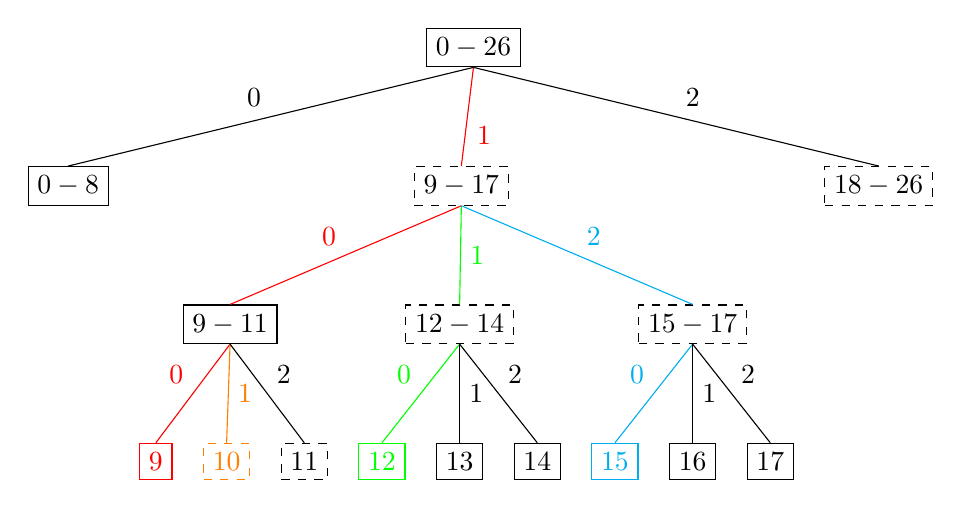
\begin{tikzpicture}[level distance=50pt, sibling distance=11pt]
\Tree
[.\node[draw]{$0-26$}; 
	\edge node[auto=right] {$0$};
	[.\node[draw]{$0-8$}; ]
	\edge[red] node[auto=left] {$1$};
	[.\node[dashed,draw]{$9-17$};
		\edge[red] node[auto=right] {$0$};
		[.\node[draw]{$9-11$};
			\edge[red] node[auto=right] {$0$};
			[.\node[draw,red]{$9$}; ]
			\edge[orange] node[auto=left] {$1$};
			[.\node[dashed,draw,orange]{$10$}; ]
			\edge node[auto=left] {$2$};
			[.\node[dashed,draw]{$11$}; ] ]
		\edge[green] node[auto=left] {$1$};
		[.\node[dashed,draw]{$12-14$};
			\edge[green] node[auto=right] {$0$};
			[.\node[draw,green]{$12$}; ]
			\edge node[auto=left] {$1$};
			[.\node[draw]{$13$}; ]
			\edge node[auto=left] {$2$};
			[.\node[draw]{$14$}; ] ]
		\edge[cyan] node[auto=left] {$2$};
		[.\node[dashed,draw]{$15-17$};
			\edge[cyan] node[auto=right] {$0$};
			[.\node[cyan,draw]{$15$}; ]
			\edge node[auto=left] {$1$};
			[.\node[draw]{$16$}; ]
			\edge node[auto=left] {$2$};
			[.\node[draw]{$17$}; ] ] ]
	\edge node[auto=left] {$2$};
	[.\node[dashed,draw]{$18-26$}; ] ]
\end{tikzpicture}

A $h(p(q), x)$ az a szint a fában, ameddig $p(q)$ és $x$ gyökérbe vezető útja különbözik.
A levelek szintje a $0$.
$d(p(q), x)$ a $h(p(q), x)$ szint vödrei közül kiválasztja azt, amelyiken $x$ útja áthalad.

A példában a beszínezett utak a $10$ szitálását mutatják.
Tegyük föl, hogy $p(q)=9$.
\begin{itemize}
\item Ekkor a sor pozícióját megnövelve $h(9, 10)=0$,
$d(9, 10)=2*0+1-1=0$, ami a $10$-es csúcsnak felel meg.
\item Ebben a $2$ és az $5$ prímet kell találjuk, azaz a $10$ összetett szám.
\item A $2$ visszahelyezéséhez $h(10, 12)=1$, $d(10, 12)=2*1+1-1=2$, ami a $12-14$-es csúcs.
\item Az $5$ visszahelyezéséhez $h(10, 15)=1$, $d(10, 15)=2*1+2-1=3$, ami a $15-17$-es csúcs.
\end{itemize}

\section{Implementáció}

A lisp implementáció a prefix-fát egy láncolt listával ábrázolja.
A lista a sor pozíciójának útja a levélből a gyökérbe.
A program a listát a végénél szükség szerint bővíti.
Minden listaelem az út egy csúcsa, és az abból a csúcsból a szülője felé mutató él.
Egy elem tartalmazza
\begin{itemize}
\item az él címkéjét
\item hogy van-e az útban a gyökérig még nem-nulla él
\item a fa szintjéhez tartozó vödröket
\item és a szülőt.
\end{itemize}

A vödrök is láncolt listák. Ezeknek az elemei cons párok, a pár mindkét eleme egy-egy szám. Ezek a számok is láncolt listával vannak ábrázolva a szám $a$ alapú számjegyeivel.

A pár egyik eleme a prím, ennek a listájában a számjegyek helyiértékei nőnek, és az utolsó tárolt számjegy mindig nem-nulla.
A másik szám a prím következő szitálásának helye.
Ebben a listában már csak azok a számjegyek vannak, amiket még nem vizsgált meg a sor, és számjegyek helyiértékei csökkennek, így minden szinten csak a lista elejét kell megvizsgálni.

A sor pozíciójának növelése állapotgépként van megvalósítva.
A program függvényhívásai az állapotok.
Az állapotváltás a függvényhívás elvégzése.
Az állapotfüggvények a paramétereket konstans időben megvizsgálják,
majd konstans időben előállítják egy másik állapotfüggvény hívásának paramétereit, és meghívják az új állapotot.
Az új állapot mindig tail position-ben van.

Egy szám szitálása 3 rekurzív függvényhívás.
Mindegyik rekurziónál a verem explicit ki van fejezve a függvényhívások paramétereiben.

A program r5rs scheme-ben van megírva, legalábbis a racket megeszi annak.

Az implementáció fájlai:
\begin{itemize}
\item \texttt{automaton1.scm}: az összeadás, és a vödrök tömbje, ezekről feltesszük, hogy be vannak építve az automatába.
\item \texttt{automaton2.scm}: a struktúrákat definiáló unzip/zip függvények, és egyéb segédfüggvények, mind konstans műveletigényű.
\item \texttt{automaton3.scm}: az állapotfüggvények, ezeknek a hívásait akarjuk megszámolni.
\item \texttt{primes.scm}: a prímek listája, a becslések ellenőrzéséhez kellenek
\item \texttt{counters.scm}: az állapotfüggvényekhez tartozó számlálók, és a hozzájuk tartozó becslések
\item \texttt{test.scm}: az egész cókmókot vezérli, valamilyen $n$-ig, és minden $2<=a<=10$ ellenőrzi a szitálás eredményét, és az állapotváltások számának becslést.
\end{itemize}

\section{Prímekre vonatkozó becslések}

Mertens tételei szerint
\begin{align*}
\sum_{p \le n}\frac{1}{p} \in \Theta(\ln{\ln{n}}) \\
\sum_{p \le n}\frac{\ln{p}}{p} \in \Theta(\ln{n})
\end{align*}

A prímszámtétel szerint
\begin{align*}
\sum_{p \le n}1 \in \Theta \left( \frac{n}{\ln{n}} \right)
\end{align*}

\section{Funkcionális modell}

Funkcionálisan programozunk, ami alatt valami olyat értek most, hogy a program állapota egy összetett formula, és az állapotátmenet függvény formulákról formulákra képez. Ahhoz, hogy elhiggyük, hogy ez lehetséges, feltesszük, hogy a formulaátírás műveletigénye korlátos, ha
\begin{itemize}
\item $a \in \mathbb{N}$, $a>1$
\item az $a$ alapú számrendszer két számjegyét össze tudjuk adni konstans időben, és az eredményben az átvitelt is megkapjuk
\item a formulákat a szintakszisfájukkal ábrázoljuk
\item a szintakszisfát a gyökerén keresztül érjük el
\item a lehetséges terminálisok halmaza véges
\item létezik a szintakszisfa csúcsainak kifokára korlát
\item létezik egy korlát, aminél mélyebben lévő csúcsot nem kell megvizsgálni ahhoz, hogy lehessen dönteni az állapotátmenet szabályáról
\item az állapotátmenet-függvény korlátos  számú új csúcs létrehozásával és átkötésével el tudja végezni a formula egy átírását
\item az $a$ szám ezekkel a korlátokkal összefüggésben van úgy, hogy feltesszük, hogy az $a-1$ elemű tömbök is formulák.
\end{itemize}

Az implementáció ezeknek a feltételeknek megfelel. Vizsgáljuk ennek az algoritmusnak a műveletigényét $n$-ig szitálva:
\begin{algorithm}[H]
\floatname{algorithm}{Algoritmus}
\caption{Edénysor-szita}
\begin{algorithmic}[1]
\State legyen $q$ egy új sor, $p(q)=1$
\While{$p(q)<n$}
\State $q$ pozíciójának növelése a fában felfele
\State $q$ invariánsának helyreállítása a fában lefele
\State $s \gets q$-ból eltávolított prímek
\If{$s$ üres}
	\State $q$ pozíciójának lemásolása a fában felfele
	\State a lemásolt érték megfordítása a fában lefele
	\State $s \gets \{ p(q) \}$
\EndIf
\State $s$ tartalmazza $p(q)$ összes prímosztóját
\For{$t \in s$}
	\State $(p(q)+t, t)$ beszúrása $q$-ba a fában felfele
	\State a fa helyreállítása lefele
\EndFor
\EndWhile
\end{algorithmic}
\end{algorithm}

A becslés ellenőrzéséhez az implementáció 5 számlálóban számolja a formulaátírások számát, minden formulaátírás pontosan egy számlálót növel.
\begin{itemize}
\item A \texttt{c} a megtalált prímek lemásolásának formulaátírásai.
\item Az \texttt{i} a sor pozíciójának növelésének formulaátírásai közül azok, amiket könnyű pontosan megszámolni.
\item Az \texttt{i-} a sor pozíciójának növelésének formulaátírásai közül azok, amiknek a számát becsüljük.
\item Az \texttt{r} új elemek sorba illesztésének formulaátírásai közül azok, amiket könnyű megszámolni.
\item Az \texttt{r+-} új elemek sorba illesztésének formulaátírásai közül azok, amiknek a száma becsült.
\end{itemize}

\subsection{\texttt{c}}

Egy prím lemásolása a fa pozíciójából maguknak a számjegyeknek a lemásolásából, és a ciklus végének felismeréséből áll.
A fában lefele pontosan annyi műveletet kell elvégezni a prím megfordításakor, mint amennyit felfele kellett a lemásoláshoz.
\begin{align*}
\texttt{c} =& 2 \left( \text{prímek száma } n \text{-ig} + \text{prímek számjegyeinek száma } n \text{-ig} \right) = \\
=& 2 \left( \sum_{p \le n}1 + \sum_{p \le n} \left( \lfloor \log_{a}{p} \rfloor + 1 \right) \right) \le \\
\le& 2 \left( \sum_{p \le n}1 + \sum_{p \le n} \left( \log_{a}{p} + 1 \right) \right) \le \\
\le& 2 \left( \sum_{p \le n}1 + \sum_{p \le n} \left( \log_{a}{n} + 1 \right) \right) = \\
=& 2 \sum_{p \le n}1 + 2 \left( \log_{a}{n} + 1 \right) \sum_{p \le n} 1 = \\
=& \left( 4 + 2 \log_{a}{n} \right) \sum_{p \le n}1 \\
\texttt{c} \in& \mathcal{O} \left( \left( 4 + 2 \log{n} \right) \frac{n}{\log{n}} \right)
= \mathcal{O} \left( \frac{n}{\log{n}} + n \right)
= \mathcal{O} \left( n \right)
\end{align*}

\subsection{\texttt{i}}

A sor pozíciójának növelésekor a fa számjegyeinek átírásához szükséges formulaátírásokat pontosan meg tudjuk határozni.
A kétszeres szorzó itt is a visszatérés a rekurzióból.
A negatív tag azért szükséges, mert a szitálást 2-től kezdjük.
\begin{align*}
\texttt{i} =& 2 \left( T(+^*, 1, n) - T(+^*, 1, 1) \right) \le \\
\le& 2 T(+^*, 1, n) \le \\
\le& \frac{2a}{a-1} n \\
\texttt{i} \in& \mathcal{O}(n)
\end{align*}

\subsection{\texttt{i-}}

Az invariáns helyreállításának műveletigénye is megbecsülhető az ismételt összeadással. A becsléshez úgy teszünk, mintha $n$ elérése után még a sorból az összes elemet eltávolítanánk.

A becsléshez feltesszük, hogy egy vödörbe beszúrni egy új elemet $O(1)$ műveletigényű, és a vödör elemeinek bejárása $O(n)$ időigényű.
Azaz az egy elemre eső műveletigény mindkét műveletnél $O(1)$.
Ez a nyilvánvalónak tűnő feltevés teszi lehetővé, hogy a műveleteket a megszámláláshoz átrendezhessük, és ne a végrehajtás sorrendjében vizsgáljuk.
A becslést minden prímre külön adjuk meg, az ismételt összeadással, majd ezeket összesítjük.

A prímek pozíciójának legnagyobb megváltozott helyiértékét nem kell megszámolni, az a sorba beszúrásnál van elkönyvelve, ez a negatív tag.

\begin{align*}
\texttt{i-} =& \sum_{p \le n} \left( T(+^*, p, \left\lfloor \frac{n}{p} \right\rfloor ) - \left\lfloor \frac{n}{p} \right\rfloor \right) \le \\
\le& \sum_{p \le n} T(+^*, p, \left\lfloor \frac{n}{p} \right\rfloor ) \le \\
\le& \sum_{p \le n} \left\lfloor \frac{n}{p} \right\rfloor \left( \lfloor \log_{a}{p} \rfloor + 1 + 2 \right) \le \\
\le& \sum_{p \le n} \frac{n}{p} \left( \log_{a}{p} + 3 \right) = \\
=& \sum_{p \le n} \frac{n}{p} \left( \frac{\ln{p}}{\ln{a}} + 3 \right) = \\
=& \frac{n}{\ln{a}} \sum_{p \le n} \frac{\ln{p}}{p} + 3n \sum_{p \le n} \frac{1}{p} \\
\texttt{i-} \in& \mathcal{O}(n \ln{n} + n \ln{\ln{n}}) = \mathcal{O}(n \log{n})
\end{align*}

\subsection{\texttt{r}}

Az $r$ minden prím minden sorba szúrását háromszor számolja:
\begin{itemize}
\item a \texttt{readd} meghívja a \texttt{readd-up}-ot
\item a \texttt{readd-up} meghívja a \texttt{readd-down}-t
\item a \texttt{readd-down} meghívja a \texttt{readd}-ot.
\end{itemize}
Ezen kívül még az $r$ számlálóba kerül, hogy a \texttt{readd} visszaadja a szitálás eredményét.

\begin{align*}
\texttt{r} =& n - 1 + 3 \sum_{p \le n} \left\lfloor \frac{n}{p} \right\rfloor < \\
<& n + 3 \sum_{p \le n} \frac{n}{p} = \\
=& n + 3n \sum_{p \le n} \frac{1}{p} \\
\texttt{r} \in& \mathcal{O}(n + n \ln{\ln{n}}) = \mathcal{O}(n \ln{\ln{n}})
\end{align*}

\subsection{\texttt{r-}}

A beszúrás maradék műveleteinek száma a megváltozott számjegyek számától függ.
A legnagyobb megváltozott helyiértékeket nem kell megszámolni, azok az \texttt{r}-ben már figyelembe vannak véve.
A kétszeres szorzó újra a rekurzió vermének feldolgozása miatt szükséges.
\begin{align*}
\texttt{r+-} =& 2 \sum_{p \le n} \left( T(+^*, p, \left\lfloor \frac{n}{p} \right\rfloor) - \left\lfloor \frac{n}{p} \right\rfloor) \right)
= 2 \texttt{i-} \\
\texttt{r+-} \in& \mathcal{O}(n \log{n})
\end{align*}

\subsection{\texttt{Összesen}}

A műveletigény felső becslése:
\begin{align*}
\texttt{c}+\texttt{i}+\texttt{i-}+\texttt{r}+\texttt{r+-}
\in \mathcal{O}(n + n + n \log{n} + n \log{\log{n}} + n \log{n})
= \mathcal{O}(n \log{n})
\end{align*}

Az alsó becslés:
\begin{align*}
\texttt{c}+\texttt{i}+\texttt{i-}+\texttt{r}+\texttt{r+-}
\ge& \sum_{p \le n} \left\lfloor \frac{n}{p} \right\rfloor \left( \left\lfloor \log_{a}{p} \right\rfloor + 1 \right) \ge \\
\ge& \sum_{p \le n} \left\lfloor \frac{n}{p} \right\rfloor \log_{a}{p} > \\
>& \sum_{p \le n} \left( \frac{n}{p} - 1 \right) \log_{a}{p} = \\
=& \sum_{p \le n} \left( \frac{n}{p} - 1 \right) \frac{\ln{p}}{\ln{a}} = \\
=& \frac{n}{\ln{a}} \sum_{p \le n} \frac{\ln{p}}{p} - \frac{1}{\ln{a}} \sum_{p \le n} \ln{p} \ge \\
\ge& \frac{n}{\ln{a}} \sum_{p \le n} \frac{\ln{p}}{p} - \frac{1}{\ln{a}} \sum_{p \le n} \ln{n} = \\
=& \frac{n}{\ln{a}} \sum_{p \le n} \frac{\ln{p}}{p} - \frac{\ln{n}}{\ln{a}} \sum_{p \le n} 1 \\
\texttt{c}+\texttt{i}+\texttt{i-}+\texttt{r}+\texttt{r+-}
\in& \Omega(n \log{n} - \ln{n} \frac{n}{\ln{n}}) = \Omega(n \log{n} - n) = \Omega(n \log{n})
\end{align*}

Tehát az edénysor szita műveletigénye a feltételezett funkcionális modellben $\Theta(n \log{n})$.

\section{$a\log{}{n}$ szalag modell}

Innentől csak átfutunk a leglényegesebbnek tűnő pontokon, mert különben sose lenne vége.

Most tegyük fel, hogy a funkcionális modell korlátos átírás feltevését nem tudjuk teljesíteni.
Pontosabban a fa módosítását még meg tudjuk oldani, de a prím-pozíciókat egyszerű átkötések helyett kénytelenek vagyunk egy lassú szalagra írni.
A szalagra írás és visszaolvasás költségét vegyük $\mathcal{O}(\log{n})$-nek.

Ekkor a domináns tag becslése:
\begin{align*}
& \sum_{p \le n} \left\lfloor \frac{n}{p} \right\rfloor ( \lfloor \log_{a}{p} \rfloor + 1 ) \mathcal{O}(\log{n}) \le \\
\le& \sum_{p \le n} \frac{n}{p} ( \log_{a}{p} + 1 ) \mathcal{O}(\log{n}) = \\
=& \mathcal{O}(\log{n}) \left( \frac{n}{\ln{n}} \sum_{p \le n} \frac{\ln{p}}{p} + n \sum_{p \le n} \frac{1}{p} \right) \in \\
\in& \mathcal{O}(\log{n}(n \log{n} + n \log{\log{n}})) = \\
= & \mathcal{O}(n \log^{2}{n})
\end{align*}

\section{Minden konstans időben modell}

Most tegyük fel, hogy nagy számokat is össze tudunk adni konstans műveletigénnyel, valamint vödrök nagy tömbjeit is tudjuk konstans időben manipulálni.
A szita tömbökön kívüli része hasonlít egy veremautomatára.

\subsection{Vegyes számrendszer}

Az ismételt összeadás műveletigényének becslése átírható vegyes számrendszerbe.
Az 1 ismételt összeadásának becsléséhez elég, ha minden helyiérték legalább olyan gyorsan nő, mint kettes alapú számrendszerben.
Valamilyen $t$ ismételt összeadásának műveletigényének becsléséhez csak $t$ számjegyeinek száma szükséges.

Tegyük fel, hogy a számrendszerben egy $n \in \mathbb{N}$ szám számjegyeinek száma $\mathcal{O}(\log{\log{n}})$. Ekkor
\begin{align*}
\sum_{p \le n} T(+^*, p, \left\lfloor \frac{n}{p} \right\rfloor)
\in& \mathcal{O}( \sum_{p \le n} \frac{n}{p} \log{\log{p}} )
\subseteq \mathcal{O}( \sum_{p \le n} \frac{n}{p} \log{\log{n}} ) = \\
=& \mathcal{O}( n \log{\log{n}} \sum_{p \le n} \frac{1}{p} )
= \mathcal{O}( n \log^{2}{\log{n}} )
\end{align*}

Adjunk meg egy ilyen számrendszert. Legyen
\begin{align*}
1 < n \in \mathbb{N} \\
m \in \mathbb{N} \\
1 < a \in \mathbb{N} \\
n_i \in \mathbb{N}_0 (i \in \mathbb{N}_0) \\
n_0 < a \\
n_i < \frac{a^{a^{i}}}{a^{a^{i-1}}} = a^{a^{i}-a^{i-1}} = a^{a^{i-1} (a-1)} (i \in \mathbb{N}^+) \\
n_m \not= 0\\
n = n_0 + \sum_{i=1}^{m} n_i a^{a^{i-1}}
\end{align*}
Ekkor
\begin{align*}
\log_{a}{\log_{a}{n}}
\ge \log_{a}{\log_{a}{n_m a^{a^m}}}
\ge \log_{a}{\log_{a}{a^{a^m}}}
= \log_{a}{a^m}
= m \\
n\text{ számjegyeinek száma} = m + 1 \in \mathcal{O}(\log{\log{n}})
\end{align*}

\subsection{Rögzített $n$-ig}

Legyen $a, t \in \mathbb{N}^+$, $a > 1$, $n = a^t$.
Ekkor
\begin{align*}
& \sum_{p \le n} T(+^*, p, \left\lfloor \frac{n}{p} \right\rfloor ) \le \\
\le& \sum_{p \le n} \left\lfloor \frac{n}{p} \right\rfloor ( \lfloor \log_{a}{p} \rfloor + 2 ) \le \\
\le& \sum_{p \le n} \frac{n}{p} ( \log_{a}{n} + 2 ) = \\
=& \sum_{p \le n} \frac{n}{p} ( \log_{a}{a^t} + 2 ) = \\
=& n (t+2) \sum_{p \le n} \frac{1}{p} \in \\
\in & \mathcal{O}(n \log{\log{n}})
\end{align*}

\section{Tárigény}

Az inkrementális szitáknál $n$-ig szitálva a sorba a prímeket $n$-ig kell tárolni, és a pozíciók felső korlátja $2n$. A prím-pozíció párok tárolásához $\mathcal{O}(n)$ bitre van szükség.

Egy fix $a$ alapú számrendszerben a szükséges vödrök száma
\begin{align*}
(a-1) (\lfloor \log_{a}{2n} \rfloor +1 ) \in \mathcal{O}(a \log_{a}{n})
\end{align*}

Rögzített $n$-ig szitálva a prímeket elég $\sqrt{n}$-ig tárolni, és a legnagyobb pozíció $n+\sqrt{n}$ lehet.
Legyen $t \in \mathbb{N}$, és $a^t = n$. Ekkor
\begin{align*}
\mathcal{O}(a \log_{a}{n}) = \mathcal{O}(t \sqrt[t]{n})
\end{align*}

A vegyes számrendszer példájában:
\begin{align*}
m =& 2n \text{ számjegyeinek száma} \\
m \le& \log_{a}{\log_{a}{2n}} \\
& a-1 + \sum_{i=1}^{m} \left( a^{a^{i-1}(a-1)} - 1 \right) < \\
<& a + \sum_{i=1}^{m} a^{a^{i}} \le \\
\le& a + \sum_{i=0}^{a^m} a^i < \\
<& a+ a a^{a^m} \le \\
\le& a+ a a^{a^{\log_{a}{\log_{a}{2n}}}} = \\
=& a+2an \in \mathcal{O}(an)
\end{align*}
Ez egy nagyon durva becslés.

\section{Cache}

Erről szívesen mondanék valamit, de nem is tudom, hogyan kéne nekifogni.

Írtam egy nagyon egyszerű, imperatív edényszitát, és azt számolom, hogy hányszor kell lassú tárba tegyek egy elemet.
Ez a \texttt{cache.scm}-ben van.
A modellem az, hogy van megadott számú gyors cons cell, és szokás szerint végtelen sorozata végtelen vödröknek, de ezekbe a vödrökbe írni és olvasni is lassú.
Ehhez a modellhez azt a cache stratégiát választottam, hogy:
\begin{itemize}
\item minden vödörhöz tartozik egy szám, hogy hány gyors cons cell van a vödörhöz rendelve
\item egy vödör olvasásakor
\begin{itemize}
\item feldolgozom a gyors cellákat, és a feldolgozással együtt vissza is fűzöm a szabadlistára
\item feldolgozom a lassú vödröt, és növelem minden elemre a lassú számlálót
\end{itemize}
\item íráskor
\begin{itemize}
\item ha van szabad gyors cella, akkor azt a vödörhöz rendelem
\item ha nincs szabad cella, de van gyors cella egy nagyobb indexű vödörhöz rendelve, akkor a legnagyobb indexű gyors cellát tartalmazó vödör egy celláját átcsoportosítom
\begin{itemize}
\item kiírom a lassú vödörbe
\item növelem a számlálót
\item hozzárendele a cellát az új vödörhöz
\end{itemize}
\item ha nincs szabad cella, és nincs nagyobb indexű vödörhöz gyors cella rendelve, akkor növelem a számlálót és a vödörbe írom az elemet
\end{itemize}
\end{itemize}

Ez a stratégia elég egyszerű, és talán optimális is ebben az elképzelt helyzetben.
Ha egy elemet egy vödörbe tesz a szita, akkor azt már beláttuk, hogy ezt az elemet minden olyan elemnél hamarabb ki is veszi a vödörből, ami éppen a sorban van, és nagyobb indexű vödörben van.

Ha tudnék valami értelmeset a mérés eredményéről nyilatkozni, akkor talán a belátásán is tudnák dolgozni. Addig is színes görbék.

\begin{figure}[H]
\renewcommand\arraystretch{1.2}
\centering
\caption{Lassú vödörelérések, $a=2$, $n=10^6$}
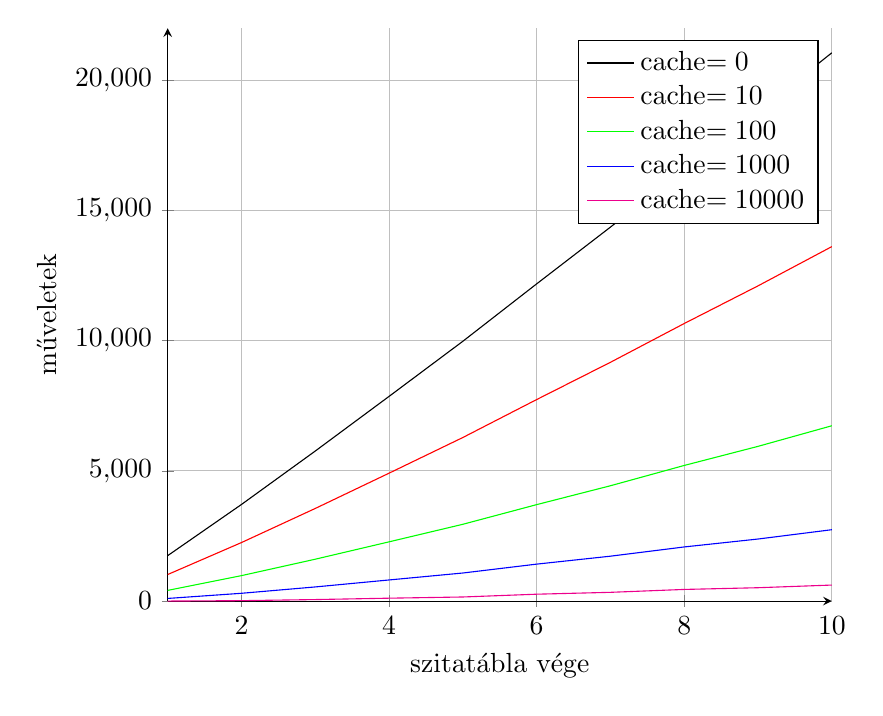
\begin{tikzpicture}
\begin{axis}[%
scale only axis,
xmin=1, xmax=10,
xlabel={szitatábla vége},
xmajorgrids,
ymin=0, ymax=22000,scaled y ticks={base 10:0},
ylabel={műveletek},
ymajorgrids,
axis lines=left,
title={ },
legend style={nodes=right}]
\addplot [
color=black
] coordinates {(1,1744)(2,3710)(3,5762)(4,7861)(5,9978)(6,12182)(7,14362)(8,16602)(9,18798)(10,21057)};
\addlegendentry{cache$=0$};
\addplot [
color=red
] coordinates {(1,1019)(2,2247)(3,3557)(4,4912)(5,6282)(6,7739)(7,9170)(8,10660)(9,12106)(10,13613)};
\addlegendentry{cache$=10$};
\addplot [
color=green
] coordinates {(1,410)(2,977)(3,1608)(4,2275)(5,2949)(6,3704)(7,4429)(8,5209)(9,5942)(10,6733)};
\addlegendentry{cache$=100$};
\addplot [
color=blue
] coordinates {(1,101)(2,299)(3,543)(4,811)(5,1078)(6,1419)(7,1724)(8,2079)(9,2383)(10,2741)};
\addlegendentry{cache$=1000$};
\addplot [
color=magenta
] coordinates {(1,0)(2,16)(3,58)(4,111)(5,157)(6,264)(7,336)(8,447)(9,513)(10,615)};
\addlegendentry{cache$=10000$};

\end{axis}
\end{tikzpicture}
\end{figure}

\begin{figure}[H]
\renewcommand\arraystretch{1.2}
\centering
\caption{Lassú vödörelérések, $a=2$, $n=10^6$}
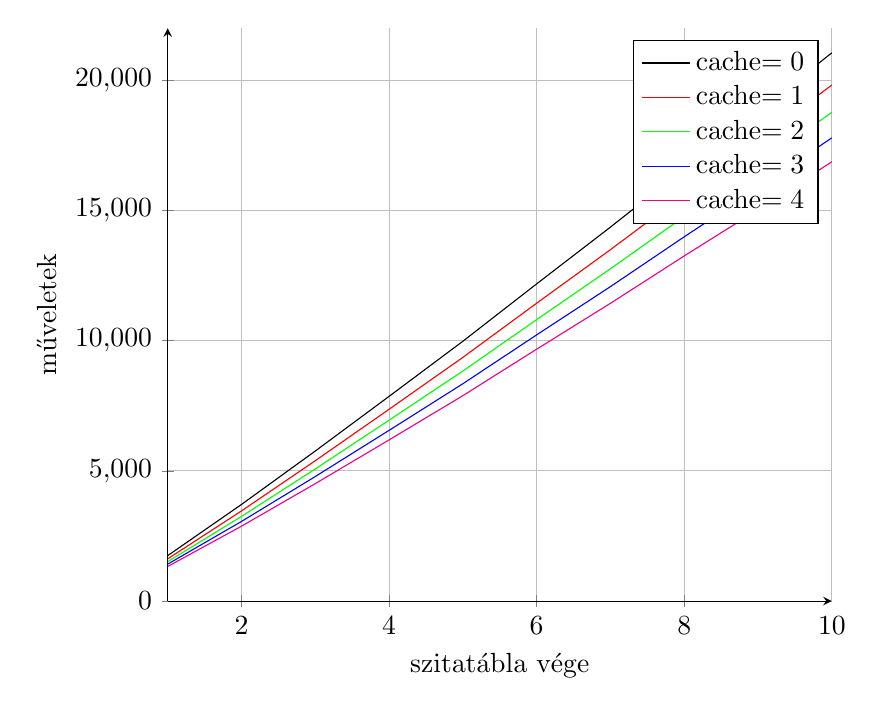
\begin{tikzpicture}
\begin{axis}[%
scale only axis,
xmin=1, xmax=10,
xlabel={szitatábla vége},
xmajorgrids,
ymin=0, ymax=22000,scaled y ticks={base 10:0},
ylabel={műveletek},
ymajorgrids,
axis lines=left,
title={ },
legend style={nodes=right}]
\addplot [
color=black
] coordinates {(1,1744)(2,3710)(3,5762)(4,7861)(5,9978)(6,12182)(7,14362)(8,16602)(9,18798)(10,21057)};
\addlegendentry{cache$=0$};
\addplot [
color=red
] coordinates {(1,1621)(2,3463)(3,5391)(4,7367)(5,9360)(6,11441)(7,13497)(8,15614)(9,17687)(10,19821)};
\addlegendentry{cache$=1$};
\addplot [
color=green
] coordinates {(1,1516)(2,3253)(3,5076)(4,6948)(5,8836)(6,10812)(7,12763)(8,14775)(9,16743)(10,18773)};
\addlegendentry{cache$=2$};
\addplot [
color=blue
] coordinates {(1,1418)(2,3058)(3,4783)(4,6556)(5,8347)(6,10224)(7,12077)(8,13991)(9,15860)(10,17792)};
\addlegendentry{cache$=3$};
\addplot [
color=magenta
] coordinates {(1,1328)(2,2877)(3,4510)(4,6191)(5,7889)(6,9675)(7,11436)(8,13257)(9,15034)(10,16873)};
\addlegendentry{cache$=4$};

\end{axis}
\end{tikzpicture}
\end{figure}

\begin{figure}[H]
\renewcommand\arraystretch{1.2}
\centering
\caption{Lassú vödörelérések, $a=7$, $n=10^6$}
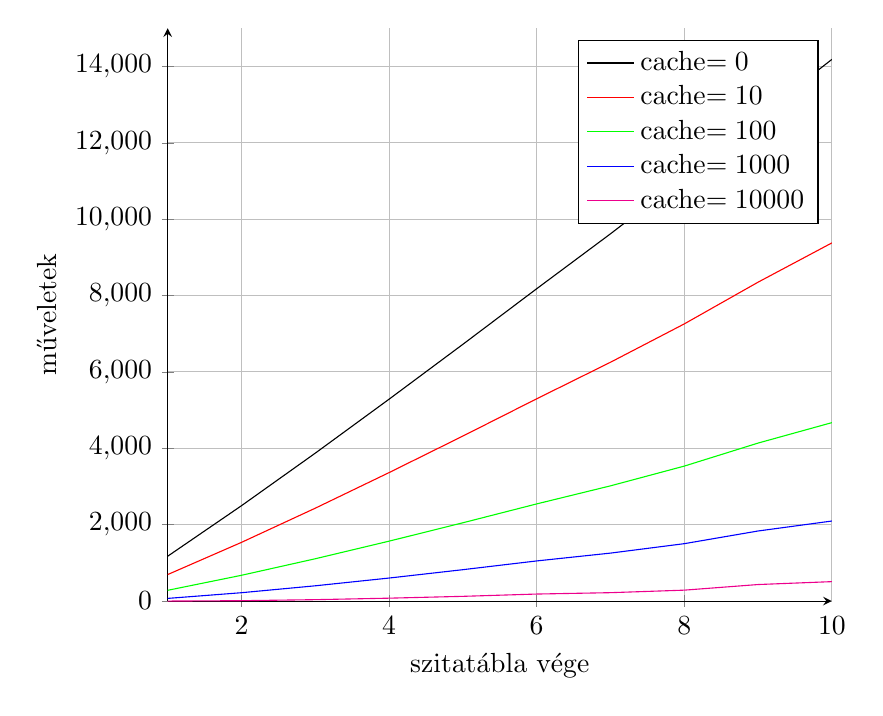
\begin{tikzpicture}
\begin{axis}[%
scale only axis,
xmin=1, xmax=10,
xlabel={szitatábla vége},
xmajorgrids,
ymin=0, ymax=15000,scaled y ticks={base 10:0},
ylabel={műveletek},
ymajorgrids,
axis lines=left,
title={ },
legend style={nodes=right}]
\addplot [
color=black
] coordinates {(1,1174)(2,2497)(3,3873)(4,5286)(5,6723)(6,8178)(7,9616)(8,11101)(9,12674)(10,14183)};
\addlegendentry{cache$=0$};
\addplot [
color=red
] coordinates {(1,694)(2,1537)(3,2432)(4,3364)(5,4321)(6,5296)(7,6253)(8,7257)(9,8350)(10,9378)
};
\addlegendentry{cache$=10$};
\addplot [
color=green
] coordinates {(1,282)(2,675)(3,1108)(4,1569)(5,2050)(6,2544)(7,3017)(8,3534)(9,4137)(10,4672)};
\addlegendentry{cache$=100$};
\addplot [
color=blue
] coordinates {(1,70)(2,219)(3,400)(4,603)(5,822)(6,1051)(7,1256)(8,1503)(9,1835)(10,2096)};
\addlegendentry{cache$=1000$};
\addplot [
color=magenta
] coordinates {(1,0)(2,10)(3,37)(4,76)(5,124)(6,184)(7,220)(8,286)(9,433)(10,509)};
\addlegendentry{cache$=10000$};

\end{axis}
\end{tikzpicture}
\end{figure}

\section{$\sqrt{n}$ vödör}

\cite{goldbach}-ban az 1.2-es algoritmus egészen jó.
Nevezzük ezt most $\sqrt{n}$ vödör algoritmusnak.
Ezzel az algoritmussal $n$-ig szitálva, $s$ nagyságú szegmenseket, $\left\lceil \frac{\sqrt{n}}{s} \right\rceil$ vödörre van szüksége.
Ezeket a vödröket egy körkörös listába szervezve hatékony sor alapú szitát kapunk.

\section{Atkin szitája}

Atkin szitájának utolsó lépése, hogy meg kell jelölni a prímek négyzeteinek többszöröseit.
$n$-ig szitálva a legnagyobb prím így is legfeljebb $\sqrt{n}$, de egy körkörös lista alapú sorhoz már $\left\lceil \frac{n}{s} \right\rceil$ vödörre lenne szükség.

\section{Összefoglalás}

\begin{table}[H]
\renewcommand\arraystretch{1.4}
\centering
\caption{Összefoglalás}
\begin{tabular}{|l|l|l|l|}
\hline
\bf{Szita} & \bf{Típus} & \bf{Idő} & \bf{Tár} \\ \cline{1-4}

$\sqrt{n}$ vödör & rögzített & $\Theta(n \log{\log{n}})$ & $\mathcal{O}(\sqrt{n}+\sqrt{n})$ \\ \cline{1-4}
Edény, lisp & inkrementális & $\Theta(n \log_{a}{n})$ & $\mathcal{O}(a \log_{a}{n} + n)$ \\\cline{1-4}
Edény, szalag & inkrementális & $\Theta(n \log_{a}^2{n})$ & $\mathcal{O}(a \log_{a}{n} + n)$ \\ \cline{1-4}
Edény, vegyes & inkrementális & $\Theta(n \log_{a}^2{\log{n}})$ & $\mathcal{O}(an + n)$ \\ \cline{1-4}
Edény, rögzített & rögzített & $\Theta(t n \log_{\sqrt[t]{n}}{\log{n}})$ & $\mathcal{O}(t \sqrt[t]{n}+\sqrt{n})$ \\ \cline{1-4}

\hline
\end{tabular}
\end{table}
\

Van-e ennek haszna? Talán. Ha az ember vödreinek overhead-je már túl nagy, megpróbálhatja edénysorral és kevesebb vödörrel. Ha Atkin szitájának többi buktatóján már túl lennék, akkor ez még előkerülhet.

Nyitott kérdések:
\begin{itemize}
\item Mi rontottam el?
\item Van-e jobb a lisp modellben?
\item Hogy néz ki egy hatékony inkrementális szita turing gépen?
\item Tudnék valamit nyilatkozni a cache-ről?
\begin{itemize}
\item Meg tudom álmodni, hogy műveletigényt a gyors/lassú kétszintű tár modellben?
\item Megfogható, hogy mi a sebességek viszonya, ha edényszitálok sok cache-sel, vagy edényszitálok cache nélkül, és direktben a kis prímek optimalizálására fordítom a memóriát?
\end{itemize}
\end{itemize}

\begin{thebibliography}{9}

\bibitem{goldbach}
Tomás Oliveira e Silva, Siegfried Herzog and Silvio Pardi: Empirical verification of the even Goldbach conjecture and computation of prime gaps up to $4\cdot10^{18}$, Math. Comp. 83 (2014), 2033-2060

\end{thebibliography}

\end{document}
